\begin{frame}[shrink=2]{Giảm chiều phi tuyến: vì sao PCA chưa đủ?}
    \small
    {\large\textcolor{your_color}{\textbf{PCA phù hợp khi dữ liệu nằm gần một cấu trúc tuyến tính.}}}

    \vspace{0.12cm}
    Với dữ liệu nằm gần một \textbf{manifold cong}, quan hệ hình học nội tại không còn được mô tả tốt bởi một không gian con tuyến tính.

    \vspace{0.14cm}
    \begin{columns}[T,onlytextwidth]
        \begin{column}{0.42\textwidth}
            \[
                \begin{aligned}
                    x_i &= f(z_i), \qquad z_i \in \mathbb{R}^d,\ d \ll p, \\
                    d_E(x_i,x_j) &\not\approx d_{\mathcal M}(x_i,x_j).
                \end{aligned}
            \]

            PCA tối ưu theo phương sai Euclid toàn cục nên phù hợp khi dữ liệu gần một không gian con tuyến tính.

            \vspace{0.1cm}
            Với dữ liệu phi tuyến, điều cần bảo toàn thường là \textbf{lân cận cục bộ}, \textbf{khoảng cách nội tại} hoặc trực tiếp hơn là \textbf{cấu trúc manifold}.
        \end{column}

        \begin{column}{0.54\textwidth}
            \begin{columns}[T,onlytextwidth]
                \begin{column}{0.49\textwidth}
                    \centering
                    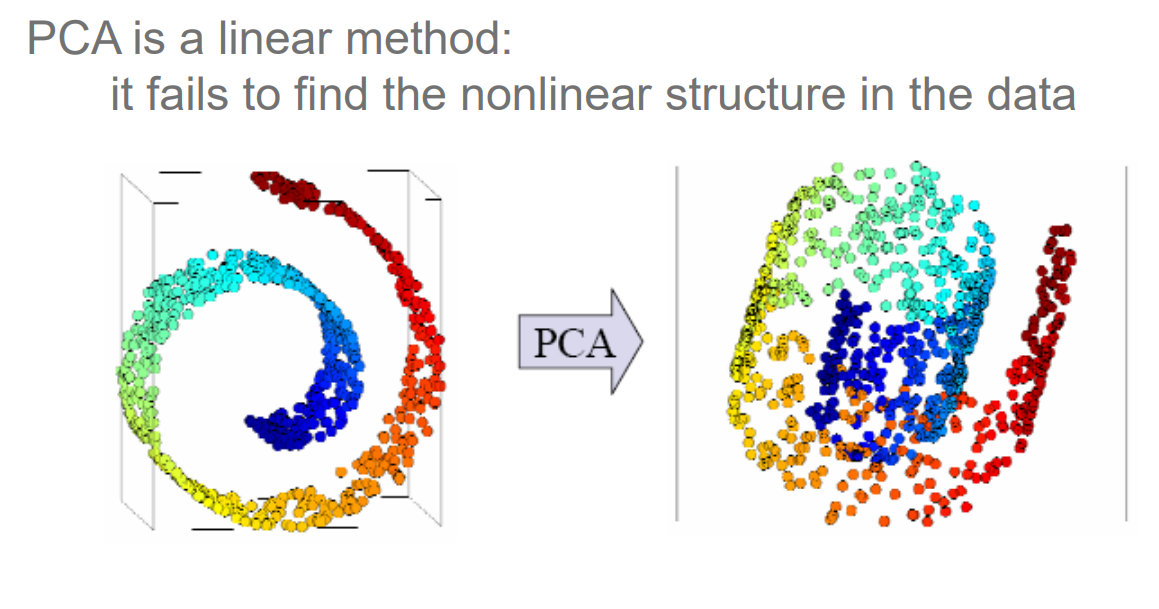
\includegraphics[width=\linewidth,height=3.15cm,keepaspectratio]{img/PCA_fails.png}
                \end{column}
                \begin{column}{0.49\textwidth}
                    \centering
                    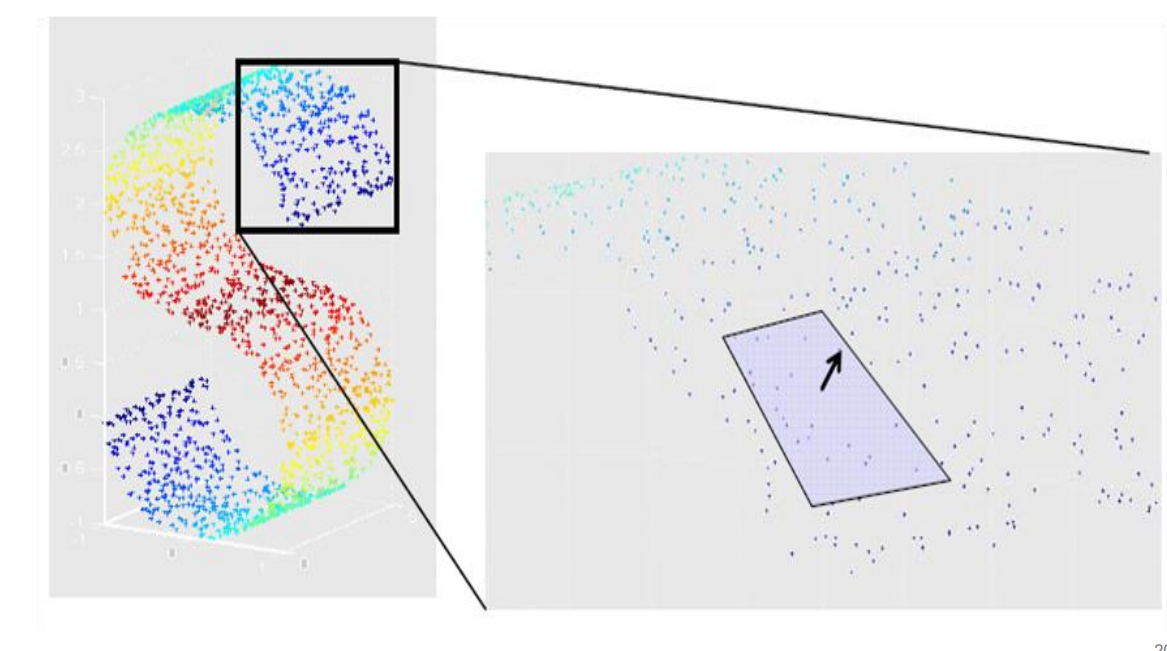
\includegraphics[width=\linewidth,height=3.15cm,keepaspectratio]{img/the Swiss-role Dataset.png}
                \end{column}
            \end{columns}

            \vspace{0.1cm}
            {\scriptsize Bên trái, phép chiếu tuyến tính có thể làm chồng lấn các nhánh phi tuyến; bên phải, manifold learning tìm cách ``trải phẳng'' cấu trúc cong nhưng vẫn giữ lại quan hệ nội tại.}
        \end{column}
    \end{columns}

    \vspace{0.08cm}
    Vì vậy, mục tiêu của giảm chiều phi tuyến không chỉ là tìm phép chiếu có phương sai lớn, mà là xây dựng embedding thấp chiều vẫn bảo toàn được hình học quan trọng của dữ liệu gốc.

    \hfill{\scriptsize Theo \cite{duchesnay2021statsml,tenenbaum2000global}}
\end{frame}

\begin{frame}[shrink=10]{Trực giác hình học: manifold, Euclid và geodesic}
    \begin{columns}[T]
        \begin{column}{0.54\textwidth}
            {\bfseries Giả thiết manifold}
            \[
                x = f(z), \qquad x \in \mathbb{R}^{P},\; z \in \mathbb{R}^{d},\; d \ll P
            \]
            Dữ liệu quan sát nhìn có vẻ cao chiều nhưng thực chất tập trung gần một cấu trúc nội tại thấp chiều hơn nhiều.

            \vspace{0.25cm}
            {\bfseries Euclid và geodesic khác nhau ở đâu?}

            \renewcommand{\arraystretch}{1.2}
            \begin{tabular}{p{0.24\linewidth} p{0.65\linewidth}}
                \toprule
                \textbf{Euclid} & Đường thẳng ngắn nhất xuyên qua không gian ambient \\
                \textbf{Geodesic} & Đường đi ngắn nhất \textbf{dọc theo bề mặt manifold} \\
                \bottomrule
            \end{tabular}

            \vspace{0.2cm}
            {\small\textcolor{your_color}{\textbf{Ý chính:}} Hai điểm có thể gần theo Euclid nhưng lại xa theo geodesic, vì vậy manifold learning thường phù hợp hơn PCA cho dữ liệu cong.}
        \end{column}

        \begin{column}{0.42\textwidth}
            \begin{figure}
                \centering
                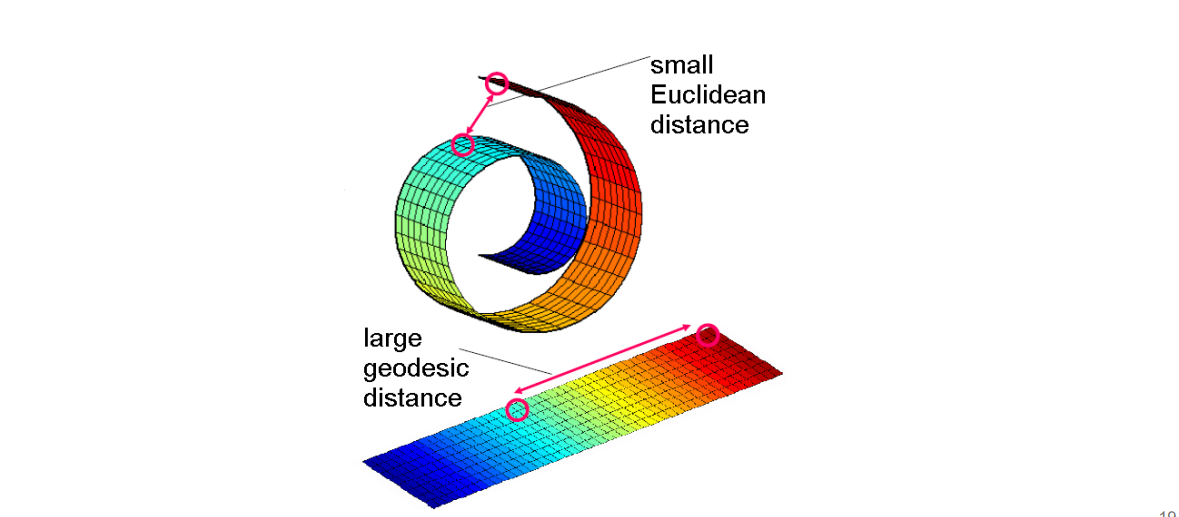
\includegraphics[width=\linewidth,height=5.5cm,keepaspectratio]{img/geodesic_distance.png}

                \vspace{0.08cm}
                {\scriptsize Đường thẳng ngắn chưa chắc là khoảng cách nội tại đúng.}
            \end{figure}
        \end{column}
    \end{columns}
\end{frame}

\begin{frame}[shrink=12]{Phát biểu bài toán và khung tính toán chung}
    Với $N$ điểm dữ liệu $\{x_i\}_{i=1}^N \subset \mathbb{R}^{P}$, mục tiêu là tìm embedding $\{z_i\}_{i=1}^N \subset \mathbb{R}^{d}$, $d \ll P$, sao cho embedding thấp chiều vẫn bảo toàn tốt nhất cấu trúc hình học nội tại của dữ liệu.

    \vspace{0.18cm}
    Một cách khái quát, hầu hết các phương pháp đều có thể viết dưới dạng
    \[
        \mathbf{Z}^{\star}
        =
        \arg\min_{\mathbf{Z}\in\mathbb{R}^{N\times d}}
        \mathcal{L}\big(\mathcal{S}_X,\mathcal{S}_Z\big),
    \]
    trong đó $\mathcal{S}_X$ là cấu trúc được trích từ dữ liệu gốc và $\mathcal{S}_Z$ là cấu trúc tương ứng trong embedding.

    \vspace{0.18cm}
    \begin{columns}[T]
        \begin{column}{0.31\textwidth}
            {\large\textcolor{your_color}{\textbf{1}}}

            {\bfseries Biểu diễn cấu trúc}

            Dữ liệu được mô tả bởi ma trận khoảng cách $\mathbf{D}$, đồ thị lân cận $k$-NN hoặc phân bố xác suất $P=[p_{ij}]$.
        \end{column}

        \begin{column}{0.31\textwidth}
            {\large\textcolor{your_color}{\textbf{2}}}

            {\bfseries Chọn tiêu chí tối ưu}

            Hàm mục tiêu đo sai khác giữa cấu trúc gốc và cấu trúc sau chiếu: \textbf{stress} trong MDS, geodesic stress trong Isomap, hay \textbf{KL divergence} trong t-SNE.
        \end{column}

        \begin{column}{0.31\textwidth}
            {\large\textcolor{your_color}{\textbf{3}}}

            {\bfseries Tìm embedding}

            Bài toán sau cùng được giải bằng nghiệm phổ hoặc tối ưu lặp, tùy theo dạng toán học của $\mathcal{L}$.
        \end{column}
    \end{columns}
\end{frame}

\begin{frame}[shrink=7]{Tiêu chí đánh giá: cấu trúc toàn cục}
    Với các phương pháp nhấn mạnh hình học toàn cục, dữ liệu thường được nhìn qua ma trận khoảng cách gốc $D=[d_{ij}]$ và ma trận khoảng cách trong embedding $\hat D=[\hat d_{ij}]$, với $\hat d_{ij}=\|z_i-z_j\|$. Khi đó, bài toán đánh giá trở thành đo mức độ gần nhau giữa hai cấu trúc khoảng cách này.

    \vspace{0.2cm}
    \begin{columns}[T,onlytextwidth]
        \begin{column}{0.48\textwidth}
            {\bfseries Stress}

            \[
                \mathrm{Stress}(Z)=
                \sqrt{\frac{\sum_{i<j}(d_{ij}-\hat d_{ij})^2}{\sum_{i<j} d_{ij}^2}}
            \]
            {\small Đo sai lệch trực tiếp giữa các khoảng cách cặp điểm trong dữ liệu gốc và trong embedding.}
        \end{column}

        \begin{column}{0.48\textwidth}
            {\bfseries Residual Variance}

            \[
                \mathrm{RV}=1-\mathrm{corr}(D,\hat D)^2
            \]
            {\small Đo phần cấu trúc tương quan giữa $D$ và $\hat D$ chưa được giải thích.}
        \end{column}
    \end{columns}

    \vspace{0.12cm}
    \begin{block}{Nguyên tắc chọn metric}
        \small
        Hai đại lượng này càng nhỏ thì embedding càng bảo toàn tốt cấu trúc toàn cục; đây là nhóm tiêu chí phù hợp nhất để đọc kết quả của \textbf{MDS} và \textbf{Isomap}.
    \end{block}
\end{frame}

\begin{frame}[shrink=8]{Tiêu chí đánh giá: cấu trúc cục bộ}
    Nếu dữ liệu được mô tả qua đồ thị $k$-NN hoặc xác suất lân cận, metric đánh giá cũng phải phản ánh đúng cấu trúc đó thay vì chỉ nhìn vào sai số khoảng cách toàn cục. Đây là quan điểm phù hợp hơn với các phương pháp ưu tiên láng giềng gần như \textbf{t-SNE}.

    \vspace{0.18cm}
    \begin{columns}[T]
        \begin{column}{0.5\textwidth}
            {\bfseries Trustworthiness}
            \[
                T(k)=1-\frac{2}{Nk(2N-3k-1)}
                \sum_{i=1}^N\sum_{j\in U_k(i)}(r(i,j)-k)
            \]
            {\small Đo mức độ embedding tránh tạo ra các \textit{false neighbors}; càng lớn càng tốt.}
        \end{column}

        \begin{column}{0.46\textwidth}
            {\bfseries k-NN Preservation}
            \[
                P@k=\frac{1}{N}\sum_{i=1}^{N}\frac{|N_k^X(i)\cap N_k^Z(i)|}{k}
            \]
            {\small Đo tỉ lệ láng giềng gốc còn được giữ sau giảm chiều; càng lớn càng tốt.}
        \end{column}
    \end{columns}

    \vspace{0.18cm}
    \begin{block}{Nguyên tắc chọn metric}
        \small
        Nếu mục tiêu là khôi phục hình học toàn cục, nên ưu tiên các tiêu chí dựa trên khoảng cách hoặc geodesic. Nếu mục tiêu là trực quan hóa cụm, các tiêu chí dựa trên lân cận cục bộ sẽ phù hợp hơn. Vì vậy, lựa chọn phương pháp cần nhất quán với \textbf{biểu diễn dữ liệu}, \textbf{hàm mục tiêu} và \textbf{metric đánh giá}.
    \end{block}
\end{frame}

\begin{frame}[shrink=4]{MDS: phát biểu bài toán}
    \small
    Với ma trận bất tương đồng $\mathbf{D}=[d_{ij}]$, mục tiêu là tìm embedding $\mathbf{z}_1,\ldots,\mathbf{z}_N\in\mathbb{R}^d$ sao cho khoảng cách trong không gian thấp chiều
    \[
        \hat d_{ij}=\|\mathbf{z}_i-\mathbf{z}_j\|
    \]
    xấp xỉ tốt nhất bất tương đồng ban đầu $d_{ij}$. Vì vậy, MDS không nhất thiết cần tọa độ gốc; đầu vào có thể chỉ là \textbf{distance matrix} hoặc \textbf{dissimilarity matrix}.

    \vspace{0.12cm}
    {\bfseries Hàm mục tiêu cơ bản}
    \[
        \mathrm{stress}(\mathbf{Z})
        =
        \sum_{i\neq j}\left(d_{ij}-\hat d_{ij}\right)^2
        =
        \sum_{i\neq j}\left(d_{ij}-\|\mathbf{z}_i-\mathbf{z}_j\|\right)^2.
    \]

    \vspace{0.12cm}
    \begin{columns}[T,onlytextwidth]
        \begin{column}{0.48\textwidth}
            {\bfseries Ý nghĩa hình học}

            MDS là bài toán bình phương tối thiểu trực tiếp trên các khoảng cách cặp điểm. Đại lượng cần bảo toàn không phải tọa độ gốc, mà là \textbf{quan hệ bất tương đồng} giữa các điểm.
        \end{column}
        \begin{column}{0.48\textwidth}
            {\bfseries Khi nào phù hợp?}

            Phương pháp này phù hợp khi mục tiêu là bảo toàn \textbf{cấu trúc khoảng cách toàn cục}; trong thực hành, chất lượng embedding thường được đọc qua \textit{stress} hoặc \textit{residual variance}.
        \end{column}
    \end{columns}

    \hfill{\scriptsize \cite{duchesnay2021statsml}}
\end{frame}

\begin{frame}[shrink=4]{Classical MDS: các bước tính toán}
    \small
    Classical MDS biến bài toán từ không gian khoảng cách sang không gian tích vô hướng, nhờ đó thu được nghiệm giải tích thay vì phải tối ưu lặp.

    \vspace{0.12cm}
    {\bfseries Bước 1: Bình phương ma trận khoảng cách}
    \[
        \mathbf{D}^{(2)}=[d_{ij}^2].
    \]

    {\bfseries Bước 2: Tâm hóa kép để thu ma trận Gram}
    \[
        \mathbf{H}=\mathbf{I}-\frac{1}{N}\mathbf{1}\mathbf{1}^T,
        \qquad
        \mathbf{B}=-\frac{1}{2}\mathbf{H}\mathbf{D}^{(2)}\mathbf{H}.
    \]
    Khi đó, $\mathbf{B}$ đóng vai trò ma trận tích vô hướng tâm hóa, với phần tử $b_{ij}=\langle \mathbf{z}_i,\mathbf{z}_j\rangle$ trong một cấu hình Euclid tương ứng.

    \vspace{0.12cm}
    {\bfseries Bước 3: Phân tích phổ}
    \[
        \mathbf{B}=\mathbf{U}\mathbf{\Lambda}\mathbf{U}^T,
        \qquad
        \mathbf{\Lambda}=\mathrm{diag}(\lambda_1,\ldots,\lambda_N),\ \lambda_1\ge\cdots\ge\lambda_N.
    \]

    {\bfseries Bước 4: Lấy $d$ thành phần chính}
    \[
        \mathbf{Z}=\mathbf{U}_d\mathbf{\Lambda}_d^{1/2},
    \]
    trong đó $\mathbf{U}_d$ chứa $d$ vector riêng ứng với các trị riêng dương lớn nhất và $\mathbf{\Lambda}_d^{1/2}=\mathrm{diag}(\sqrt{\lambda_1},\ldots,\sqrt{\lambda_d})$.

    \hfill{\scriptsize \cite{duchesnay2021statsml}}
\end{frame}

\begin{frame}[shrink=5]{Classical MDS: diễn giải nghiệm}
    \small
    Từ công thức
    \[
        \mathbf{B}=\mathbf{Z}\mathbf{Z}^T,
    \]
    Classical MDS khôi phục một cấu hình điểm sao cho ma trận tích vô hướng của embedding khớp tốt nhất với ma trận Gram suy ra từ khoảng cách ban đầu.

    \vspace{0.14cm}
    \begin{columns}[T,onlytextwidth]
        \begin{column}{0.48\textwidth}
            {\bfseries Tính chất của nghiệm}

            Nếu $\mathbf{B}$ là nửa xác định dương, nghiệm thu được là nghiệm đóng, tất định và không phụ thuộc khởi tạo. Embedding chỉ được xác định đến phép quay, phản xạ hoặc tịnh tiến, nhưng các khoảng cách theo cặp được giữ nguyên.
        \end{column}
        \begin{column}{0.48\textwidth}
            {\bfseries Liên hệ với PCA}

            Nếu $\mathbf{D}$ là ma trận khoảng cách Euclid suy ra từ dữ liệu gốc đã được tâm hóa, Classical MDS cho cùng không gian con chính như PCA. Vì vậy, PCA có thể xem như một trường hợp đặc biệt của MDS dưới metric Euclid.
        \end{column}
    \end{columns}

    \vspace{0.12cm}
    Trong trường hợp xuất hiện trị riêng âm, điều đó cho thấy ma trận bất tương đồng không hoàn toàn tương thích với một cấu hình Euclid; khi đó ta thường chỉ giữ các trị riêng dương lớn nhất để xây embedding xấp xỉ.

    \hfill{\scriptsize \cite{duchesnay2021statsml}}
\end{frame}

\begin{frame}[shrink=8]{Isomap: ý tưởng hình học}
    \begin{columns}[T]
        \begin{column}{0.54\textwidth}
            {\bfseries Ý tưởng cốt lõi}

            Isomap thay khoảng cách Euclid trong MDS bằng \textbf{khoảng cách geodesic} trên manifold. Về mặt lý tưởng, embedding cần thỏa
            \[
                \|\mathbf{z}_i-\mathbf{z}_j\|
                \approx
                d_{\mathcal{M}}(\mathbf{x}_i,\mathbf{x}_j)
            \]
            với $d_{\mathcal{M}}$ là khoảng cách nội tại dọc theo manifold.

            \vspace{0.15cm}
            Trong thực tế, khoảng cách này được xấp xỉ bởi
            \[
                d_{\mathcal{M}}(\mathbf{x}_i,\mathbf{x}_j)
                \approx
                d_{ij}^{G}
            \]
            trong đó $d_{ij}^{G}$ là shortest path trên đồ thị láng giềng. Về bản chất, Isomap là \textbf{classical MDS áp dụng trên ma trận khoảng cách geodesic xấp xỉ}.
        \end{column}

        \begin{column}{0.45\textwidth}
            \begin{figure}
                \centering
                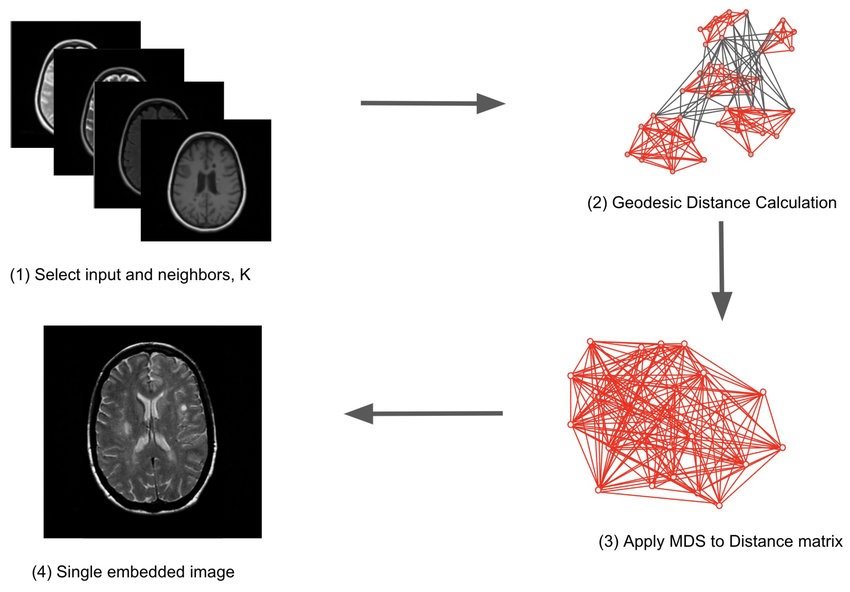
\includegraphics[width=\linewidth,height=4.7cm,keepaspectratio]{img/isomap_algorithm_pipeline.png}

                \vspace{0.08cm}
                {\scriptsize Isomap ước lượng geodesic qua shortest path trên đồ thị láng giềng.}
            \end{figure}

        \end{column}
    \end{columns}

    \hfill{\scriptsize \cite{tenenbaum2000global,duchesnay2021statsml}}
\end{frame}

\begin{frame}[shrink=8]{Isomap: quy trình và điều kiện áp dụng}
    \begin{columns}[T]
        \begin{column}{0.53\textwidth}
            {\bfseries Quy trình thuật toán}
            \begin{enumerate}
                \item Xây dựng đồ thị k-NN hoặc $\varepsilon$-graph.
                \item Gán trọng số cạnh bằng khoảng cách Euclid cục bộ.
                \item Tính shortest path giữa mọi cặp đỉnh để thu được $\mathbf{D}^G$.
                \item Chạy classical MDS trên $\mathbf{D}^G$.
            \end{enumerate}

            \vspace{0.15cm}
            {\bfseries Hàm mục tiêu ngầm ẩn}
            \[
                \sum_{i\neq j}\left(d_{ij}^{G}-\|\mathbf{z}_i-\mathbf{z}_j\|\right)^2
            \]
            tức là bảo toàn tốt nhất các khoảng cách geodesic xấp xỉ trên đồ thị lân cận.
        \end{column}

        \begin{column}{0.42\textwidth}
            \begin{block}{Điều kiện áp dụng}
                \small
                Isomap hiệu quả khi manifold trơn, liên thông và được lấy mẫu đủ dày. Nó đặc biệt phù hợp với dữ liệu dạng \emph{Swiss roll} hay \emph{S-curve}.
            \end{block}

            \begin{alertblock}{Giới hạn}
                \small
                Nếu đồ thị láng giềng bị đứt gãy, có \emph{short-circuit} do chọn $k$ quá lớn, hoặc dữ liệu quá nhiễu, xấp xỉ geodesic sẽ sai và embedding mất ý nghĩa hình học.
            \end{alertblock}
        \end{column}
    \end{columns}

    \hfill{\scriptsize \cite{tenenbaum2000global,duchesnay2021statsml}}
\end{frame}

\begin{frame}{t-SNE: mô hình xác suất cho lân cận cục bộ}
    \footnotesize
    \setlength{\abovedisplayskip}{4pt}
    \setlength{\belowdisplayskip}{4pt}
    \begin{columns}[T,onlytextwidth]
        \begin{column}{0.58\textwidth}
            {\bfseries Nguyên lý}

            t-SNE không bảo toàn trực tiếp khoảng cách toàn cục; thay vào đó, nó khớp \textbf{phân bố xác suất lân cận} giữa không gian cao chiều và embedding thấp chiều.

            \vspace{0.15cm}
            {\bfseries Xác suất trong không gian gốc}
            \[
                p_{ij}=\frac{p_{j|i}+p_{i|j}}{2N},
                \qquad
                p_{j|i}
                \propto
                \exp\!\left(-\frac{\|\mathbf{x}_i-\mathbf{x}_j\|^2}{2\sigma_i^2}\right)
            \]

            {\bfseries Xác suất trong embedding}
            \[
                q_{ij}
                =
                \frac{(1+\|\mathbf{z}_i-\mathbf{z}_j\|^2)^{-1}}
                {\sum_{k\neq l}(1+\|\mathbf{z}_k-\mathbf{z}_l\|^2)^{-1}}.
            \]

            {\bfseries Hàm mục tiêu}
            \[
                \mathcal{L}(\mathbf{Z})=\mathrm{KL}(P\|Q)
                =
                \sum_{i\neq j}p_{ij}\log\frac{p_{ij}}{q_{ij}}.
            \]
        \end{column}

        \begin{column}{0.38\textwidth}
            \centering
            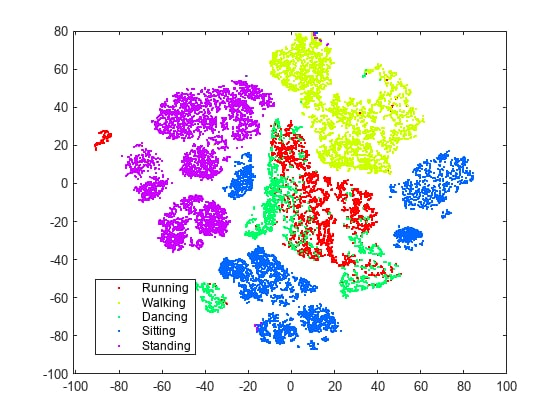
\includegraphics[width=\linewidth,height=3.15cm,keepaspectratio]{img/tsne_visualization_example.jpg}

            \vspace{0.12cm}
            {\scriptsize t-SNE làm nổi bật các cụm cục bộ và quan hệ láng giềng gần trong biểu diễn 2D/3D.}

            \vspace{0.18cm}
            {\bfseries Ý nghĩa hình học}

            \small
            Phân bố Student-\emph{t} ở không gian thấp chiều giúp giảm \emph{crowding problem}, nhờ đó các cụm cục bộ được tách rõ hơn.
        \end{column}
    \end{columns}

    \hfill{\scriptsize \cite{maaten2008visualizing,duchesnay2021statsml}}
\end{frame}

\begin{frame}[shrink=4]{t-SNE: quy trình và cách diễn giải}
    \scriptsize
    \setlength{\abovedisplayskip}{4pt}
    \setlength{\belowdisplayskip}{4pt}
    \begin{columns}[T,onlytextwidth]
        \begin{column}{0.45\textwidth}
            {\bfseries Quy trình thuật toán}

            \begin{enumerate}
                \item Từ khoảng cách trong không gian cao chiều, xây dựng các xác suất có điều kiện $p_{j|i}$.
                \item Chọn $\sigma_i$ cho từng điểm bằng \textit{binary search} sao cho entropy của $P_i$ khớp với \textit{perplexity} cho trước.
                \item Đối xứng hóa để thu được
                \[
                    p_{ij}=\frac{p_{j|i}+p_{i|j}}{2N}.
                \]
                \item Khởi tạo embedding $\mathbf{z}_i$, tính $q_{ij}$ trong không gian thấp chiều và tối ưu \(\mathrm{KL}(P\|Q)\) cho đến khi hội tụ.
            \end{enumerate}

            \vspace{0.06cm}
            {\bfseries Bản chất phương pháp}

            t-SNE được thiết kế chủ yếu cho \textbf{visualization} 2D/3D. Phương pháp này làm rõ cấu trúc cụm và quan hệ láng giềng gần, chứ không nhằm khôi phục chính xác hình học toàn cục.
        \end{column}

        \begin{column}{0.51\textwidth}
            {\bfseries Tối ưu embedding}

            Embedding được tìm bằng tối ưu lặp của KL divergence. Gradient theo từng điểm có dạng
            \[
                \frac{\partial \mathcal{L}}{\partial \mathbf{z}_i}
                =
                4\sum_j (p_{ij}-q_{ij})(\mathbf{z}_i-\mathbf{z}_j)(1+\|\mathbf{z}_i-\mathbf{z}_j\|^2)^{-1}.
            \]

            \vspace{0.1cm}
            {\bfseries Ảnh hưởng của perplexity}

            \[
                \mathrm{Perp}(P_i)=2^{H(P_i)},
                \qquad
                H(P_i)=-\sum_j p_{j|i}\log_2 p_{j|i}
            \]

            Đại lượng này xác định quy mô lân cận hiệu dụng quanh mỗi điểm: \textit{perplexity} nhỏ nhấn mạnh cấu trúc rất cục bộ, còn \textit{perplexity} lớn phản ánh lân cận rộng hơn nhưng có thể làm mờ các cụm nhỏ.

            \vspace{0.1cm}
            {\bfseries Cách đọc kết quả}

            Khoảng cách giữa các cụm trên hình 2D không nên được diễn giải quá mạnh, vì t-SNE không ưu tiên bảo toàn hình học toàn cục. Khi phân tích kết quả, nên tập trung vào các cụm cục bộ và các láng giềng gần còn được duy trì sau phép chiếu.
        \end{column}
    \end{columns}

    \hfill{\scriptsize \cite{maaten2008visualizing,duchesnay2021statsml}}
\end{frame}

\begin{frame}[shrink=10]{Chọn phương pháp nào?}
    \footnotesize
    \renewcommand{\arraystretch}{1.18}
    \begin{tabular}{p{0.16\linewidth} p{0.22\linewidth} p{0.27\linewidth} p{0.26\linewidth}}
        \toprule
        \textbf{Phương pháp} & \textbf{Bảo toàn gì?} & \textbf{Điểm mạnh} & \textbf{Nên dùng khi} \\
        \midrule
        PCA & Phương sai toàn cục & Nhanh, ổn định, dễ diễn giải & Dữ liệu gần tuyến tính hoặc cần tiền xử lý cho mô hình sau đó \\
        \addlinespace
        MDS & Khoảng cách cặp điểm & Làm việc trực tiếp với distance matrix & Đầu vào đã là ma trận khoảng cách/bất tương đồng \\
        \addlinespace
        Isomap & Khoảng cách geodesic toàn cục & Có khả năng ``trải phẳng'' manifold liên tục & Dữ liệu có cấu trúc cong như Swiss roll, S-curve \\
        \addlinespace
        t-SNE & Lân cận cục bộ, cấu trúc cụm & Trực quan hóa rất tốt & Muốn quan sát cụm và hàng xóm gần trong dữ liệu cao chiều \\
        \bottomrule
    \end{tabular}

    \vspace{0.25cm}
    \begin{center}
        \textcolor{your_color}{\textbf{Kết luận:}} PCA là lựa chọn mặc định khi cần ổn định và đơn giản; manifold learning phát huy tác dụng khi dữ liệu có cấu trúc cong hoặc khi mục tiêu chính là khám phá hình học dữ liệu.
    \end{center}
\end{frame}
